\documentclass[]{article}
\usepackage{graphicx}
\usepackage[svgnames]{xcolor} 
\usepackage{fancyhdr}

\usepackage[hidelinks]{hyperref}
\usepackage{enumitem}
\usepackage[many]{tcolorbox}
\usepackage{listings }
\usepackage[a4paper, total={6in, 8in}]{geometry}
\usepackage{afterpage}
\usepackage{amssymb}
\usepackage{pdflscape}
\usepackage{textcomp}
\usepackage{xecolor}
\usepackage{rotating}
\usepackage[Kashida]{xepersian}
\usepackage[T1]{fontenc}
\usepackage{tikz}
\usepackage[utf8]{inputenc}
\usepackage{PTSerif} 
\usepackage{seqsplit}
\usepackage{changepage}



\usepackage{listings}
\usepackage{xcolor}
\usepackage{sectsty}
 
\definecolor{codegreen}{rgb}{0,0.6,0}
\definecolor{codegray}{rgb}{0.5,0.5,0.5}
\definecolor{codepurple}{rgb}{0.58,0,0.82}
\definecolor{backcolour}{rgb}{0.95,0.95,0.92}
 
\NewDocumentCommand{\codeword}{v}{
\texttt{\textcolor{blue}{#1}}
}
\lstset{language=java,keywordstyle={\bfseries \color{blue}}}

\lstdefinestyle{mystyle}{
    backgroundcolor=\color{backcolour},   
    commentstyle=\color{codegreen},
    keywordstyle=\color{magenta},
    numberstyle=\tiny\color{codegray},
    stringstyle=\color{codepurple},
    basicstyle=\ttfamily\normalsize,
    breakatwhitespace=false,         
    breaklines=true,                 
    captionpos=b,                    
    keepspaces=true,                 
    numbers=left,                    
    numbersep=5pt,                  
    showspaces=false,                
    showstringspaces=false,
    showtabs=false,                  
    tabsize=2
}

\lstset{style=mystyle}

 \settextfont[BoldFont={XB Zar bold.ttf}]{XB Zar.ttf}


\setlatintextfont[Scale=1.0,
 BoldFont={LiberationSerif-Bold.ttf}, 
 ItalicFont={LiberationSerif-Italic.ttf}]{LiberationSerif-Regular.ttf}





\newcommand{\inputsample}[1]{
    ~\\
    \textbf{ورودی نمونه}
    ~\\
    \begin{tcolorbox}[breakable,boxrule=0pt]
        \begin{latin}
            \large{
                #1
            }
        \end{latin}
    \end{tcolorbox}
}

\newcommand{\outputsample}[1]{
    ~\\
    \textbf{خروجی نمونه}

    \begin{tcolorbox}[breakable,boxrule=0pt]
        \begin{latin}
            \large{
                #1
            }
        \end{latin}
    \end{tcolorbox}
}

\newenvironment{changemargin}[2]{%
\begin{list}{}{%
\setlength{\topsep}{0pt}%
\setlength{\leftmargin}{#1}%
\setlength{\rightmargin}{#2}%
\setlength{\listparindent}{\parindent}%
\setlength{\itemindent}{\parindent}%
\setlength{\parsep}{\parskip}%
}%
\item[]}{\end{list}}


\definecolor{foldercolor}{RGB}{124,166,198}
\definecolor{sectionColor}{HTML}{ff5e0e}
\definecolor{subsectionColor}{HTML}{008575}


\defpersianfont\titr[Scale=1.5]{Lalezar-Regular.ttf}

\sectionfont{\color{sectionColor}}  % sets colour of sections



\subsectionfont{\color{subsectionColor}}  % sets colour of sections

\renewcommand{\labelitemii}{$\circ$}


\renewcommand{\baselinestretch}{1.1}
\setlength{\parskip}{1.2pt}

\begin{document}


%%% title pages
\begin{titlepage}
\begin{center}

\textbf{ \Huge{به نام خدا} }
        
\vspace{0.2cm}


\includegraphics[width=0.4\textwidth]{sharif1.png}\\
\vspace{0.2cm}
\textbf{ \Huge{\emph درس برنامه‌سازی پیشرفته} }\\
\vspace{0.25cm}
\textbf{ \Large{ آشنایی با Trello} }
\vspace{0.2cm}
       
 
      \large \textbf{دانشکده مهندسی کامپیوتر}\\\vspace{0.1cm}
    \large   دانشگاه صنعتی شریف\\\vspace{0.2cm}
       \large   ﻧﯿﻢ سال دوم 99-98 \\\vspace{0.10cm}
      \noindent\rule[1ex]{\linewidth}{1pt}
اساتید:\\
    \textbf{{مهدی مصطفی‌زاده، ایمان عیسی‌زاده، امیر ملک‌زاده، علی چکاه}}



        \vspace{0.10cm}
نگارش و تهیه محتوا:\\
    \textbf{{یاشار ظروفچی}}
    
       \vspace{0.10cm}
       تنظیم داک:\\
    \textbf{{امیرمهدی نامجو}}

    
        \vspace{0.05cm}

\end{center}
\end{titlepage}
%%% title pages


%%% header of pages
\newpage
\pagestyle{fancy}
\fancyhf{}
\fancyfoot{}
\cfoot{\thepage}
\lhead{فاز صفر}
\rhead{
\includegraphics[width=0.1\textwidth]{sharif.png}\\
دانشکده مهندسی کامپیوتر
}
\chead{پروژه برنامه‌سازی پیشرفته}
%%% header of pages
\renewcommand{\headrulewidth}{2pt}

\KashidaOff


 \Large \textbf{\\
}


\section*{{\titr مقدمه - Trello چیست؟}}

ابزار \lr{Trello} یک نرم‌افزار تحت وب است که برای مدیریت کار (بعضا از آن به‌عنوان مدیریت پروژه نیز یاد می‌شود) به کار می‌رود. این برنامه از ساختار کانبانی تبعیت می‌کند. کلید‌واژه‌های گفته شده به مرور تبیین و توصیف می‌شوند.

نرم‌افزارهای مدیریت پروژه ابزارهایی هستند که می‌توان از آن‌ها برای برنامه ریزی، هماهنگی، همکاری و تقسیم وظایف در انجام پروژه‌ها استفاده کرد.

\begin{center}


\includegraphics[width=0.8\textwidth]{images/image9.png}

\end{center}

\newpage

\section*{{\titr ساختار Trello}}

کانبان (که در زبان ژاپنی به معنی تختهٔ اعلان است) روشی برای مدیریت و بهبود کار در سیستم‌های توسعهٔ انسانی است. این رویکرد با هدف مدیریت کردن کارها از طریق متعادل کردن تقاضا با ظرفیت‌های موجود، و همچنین بهبود عملکرد تنگناهای سطح سیستم انجام می‌شود.

تابلوهای کانبان، بر اساس محتوایی که در آن استفاده می‌شود به صورت اختصاصی طراحی می‌شوند بنابراین، به‌طور قابل توجهی با یکدیگر تمایز دارند. در مورد پیاده‌سازی این معماری موارد زیر مطرح می‌شوند:

\begin{enumerate}
\item
کارهای خود را مجسم کنید.

\item
کارهای در حال انجام را محدود کنید.

\item
سیاست‌ها را به صراحت بیان کنید.

\item
جریان کاری را مدیریت کنید.

\item
روال‌های بازخورد انجام دهید.

\item
به صورت مشارکتی پیشرفت کنید.

\end{enumerate}

یکی از نکات مهم در انجام پروژه‌های گروهی تقسیم وظایف است. \lr{Trello} ابزاری است که به این مهم کمک می‌کند. همچنین
 \lr{Pair programming} 
 نیز یکی دیگر از مواردی است که در این‌گونه پروژه‌ها  لازم است که معادل این فرض است:

هیچ \lr{task} ای پایان نخواهد پذیرفت مگر همگی به آگاهی لازم برای برخورد با آن بخش پروژه رسیده باشند.

در \lr{Trello} با قابلیت‌هایی که خواهیم دید متوجه خواهیم شد که انجام این روال‌های گفته شده تا چه حد منظم‌تر خواهد بود.

\newpage

\section*{{\titr آغاز کار با Trello}}

\begin{itemize}

\item

مانند عموم برنامه‌های تحت وب می‌بایست یک حساب کاربر در آن ایجاد کنید یا از حساب گوگل خود برای ورود استفاده کنید.

\begin{center}


\includegraphics[width=1.0\textwidth]{images/image1.png}

\end{center}

\item

پس از ساخت حساب و ورود به سایت، شما وارد صفحه‌ای می‌شود که \lr{Board} (تخته)‌ های شما نمایان است. در صورتی که تاکنون \lr{Board}ی نداشته‌اید اقدام به ساخت یک تختهٔ جدید کنید.

یک \lr{Board} می‌تواند به ۲ صورت زیر باشد:

\begin{enumerate}

\item
خصوصی یا \lr{private}؛ تنها به کسانی که شما اجازه می‌دهید امکان مشاهده داده شده است.

\item
عمومی یا \lr{public}؛ هر کسی می‌تواند تخته شما را رؤیت کند.

\end{enumerate}

\begin{center}

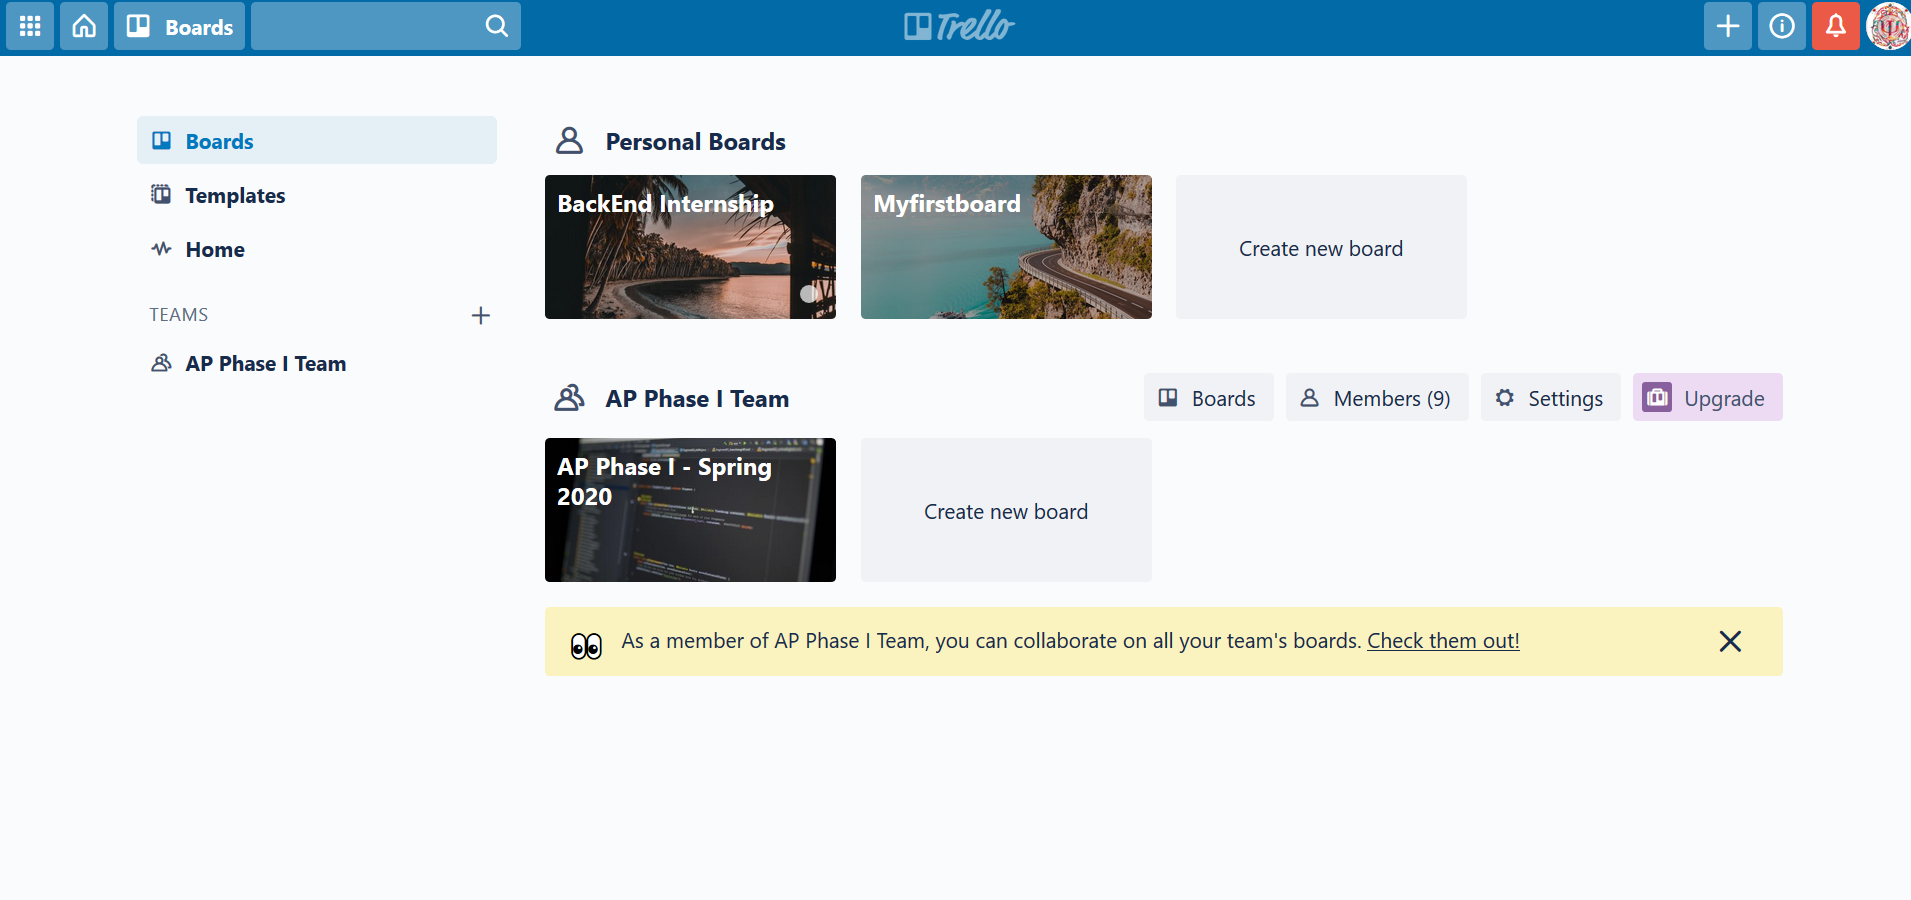
\includegraphics[width=1.0\textwidth]{images/image4.png}

\end{center}

\begin{center}

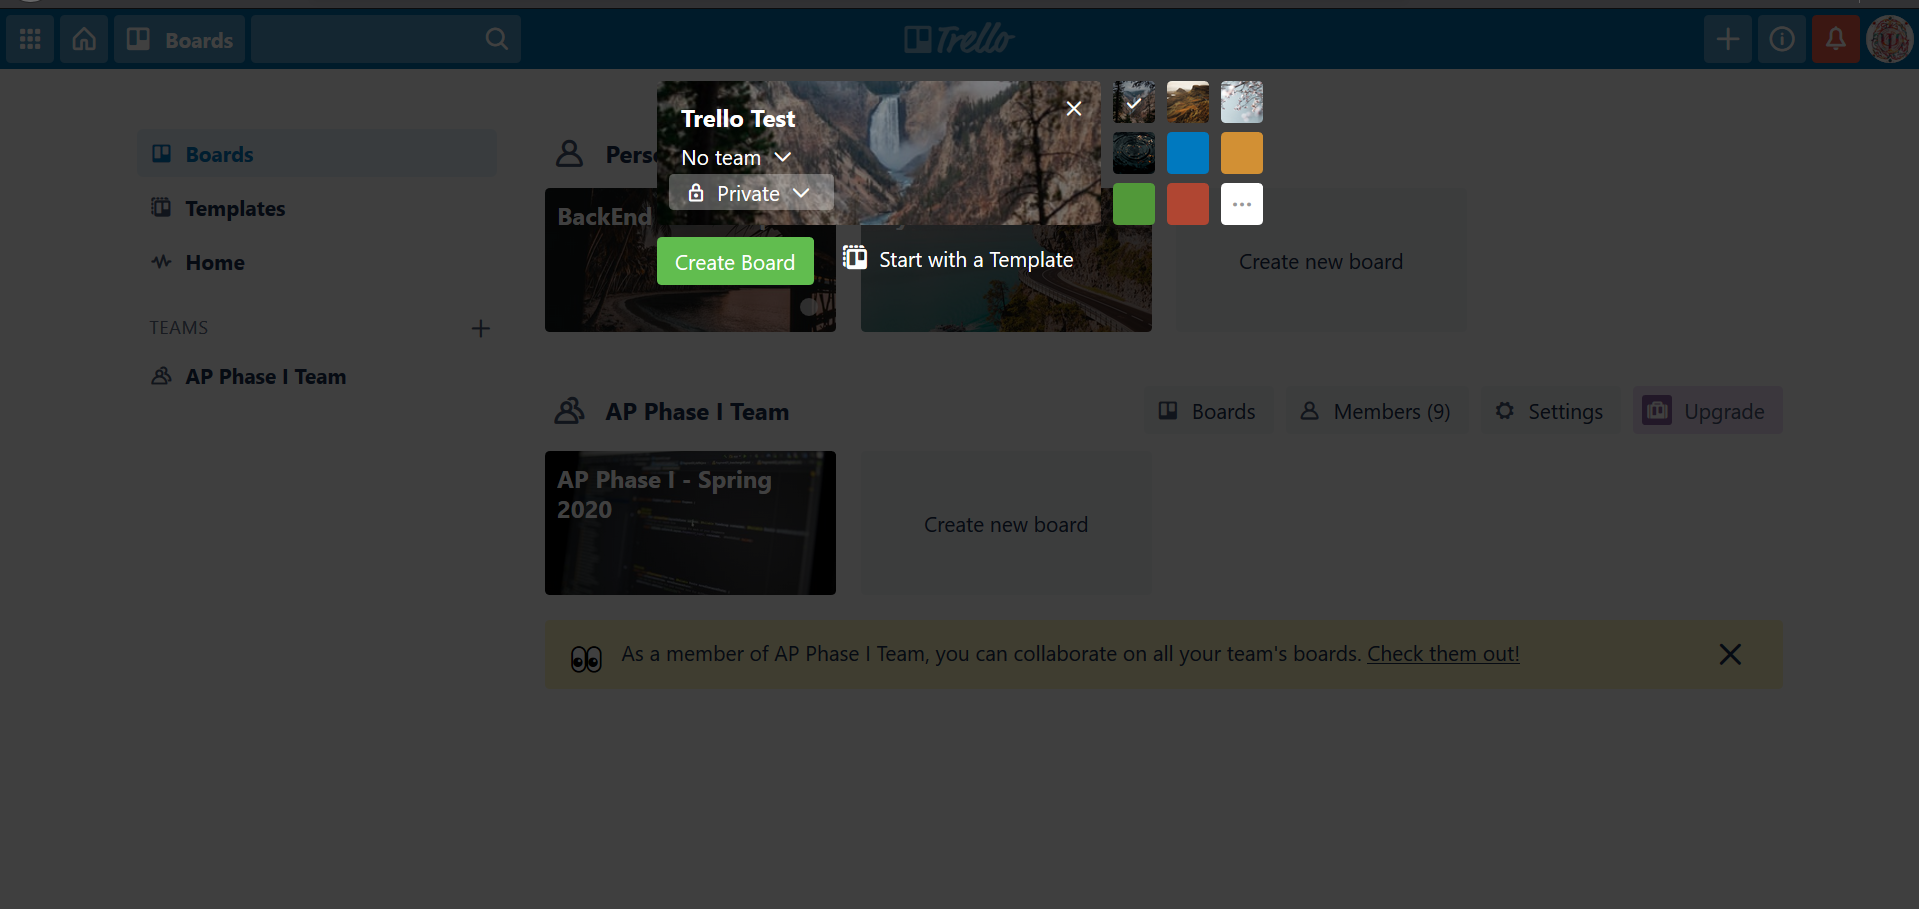
\includegraphics[width=1.0\textwidth]{images/image10.png}

\end{center}

\item

پس از ساخت \lr{Board}، اقدام به تعریف لیست‌های خود کنید. یکی از روش‌های تعریف لیست، تعیین وضعیت کار (\lr{task}) است. برای مثال: تعریف‌شده \lr{(to do)}، در حال پیگیری \lr{(doing)}، در حال بازبینی \lr{(review)} و پایان یافته \lr{(done)}. لیست‌ها باید طوری تعریف شوند که یک \lr{Card} نتواند در دو لیست قرار گیرد.

\begin{center}

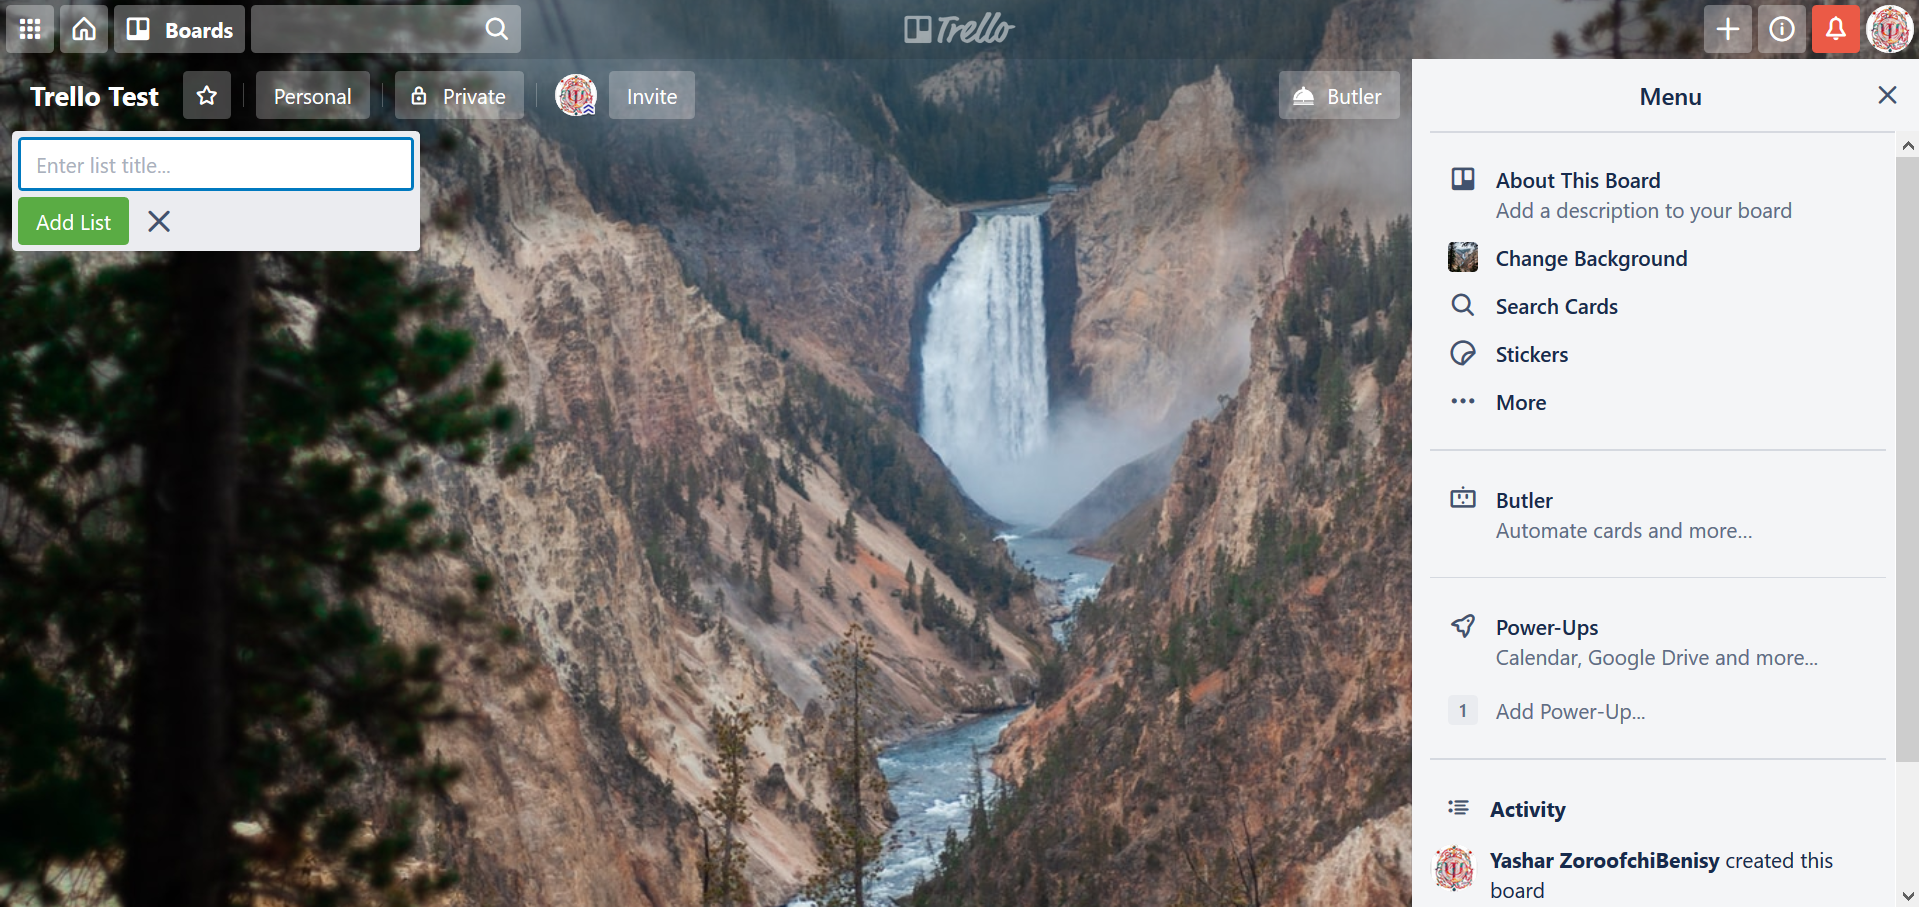
\includegraphics[width=1.0\textwidth]{images/image2.png}

\end{center}

\item

آیتم \lr{Card}، کوچکترین کار (\lr{task})ی است که استقلال خود را حفظ می‌کند. برای مثال فرض کنید یک سامانهٔ انتخاب واحد نوشته‌اید. اینکه حین برداشتن درس، در صورتی که ظرفیت داشته باشد جزو درس‌های گرفته شده رود، در صورت باز بودن ظرفیت رزرو، شما را در لیست انتظار قرار دهد وگرنه امکان اخذ واحد را از شما سلب کند، هنگام تعریف پروژه، همه تحت عنوان یک کارت «درخواست درس» قرار خواهند گرفت؛ زیرا اجزای مختلف این فرآیند در صورت ناقص بودن به هیچ‌وجه قابل قبول نخواهند بود؛ به عبارت دیگر، روال‌های گفته شده به یکدیگر وابسته‌اند و نقطهٔ گذاری بین آن‌ها نیست. ولی تعریف یک کارت تحت عنوان « طراحی و عیب‌یابی سامانهٔ انتخاب واحد » صحیح نیست. زیرا این سامانه بخش‌های مختلفی دارد که هرکدام مستقلا کاری را انجام می‌دهند. برای مثال مشاهدهٔ لیست درس‌ها ارتباطی با واحد‌های دریافت شده از نظر عملیاتی ندارد و می‌توانند مستقل از همدیگر یکی درست عمل کند و دیگر نادرست.

\begin{center}


\includegraphics[width=1.0\textwidth]{images/image8.png}

\end{center}

\item
هر \lr{Card} محتوا و اشیاء گوناگونی را می‌تواند دربرگیرد:


\begin{itemize}
\item
چک‌لسیت

\item
پیوست

\item
توضیحات

\item
شرح فعالیت

\item
برچسب

\end{itemize}

\begin{center}

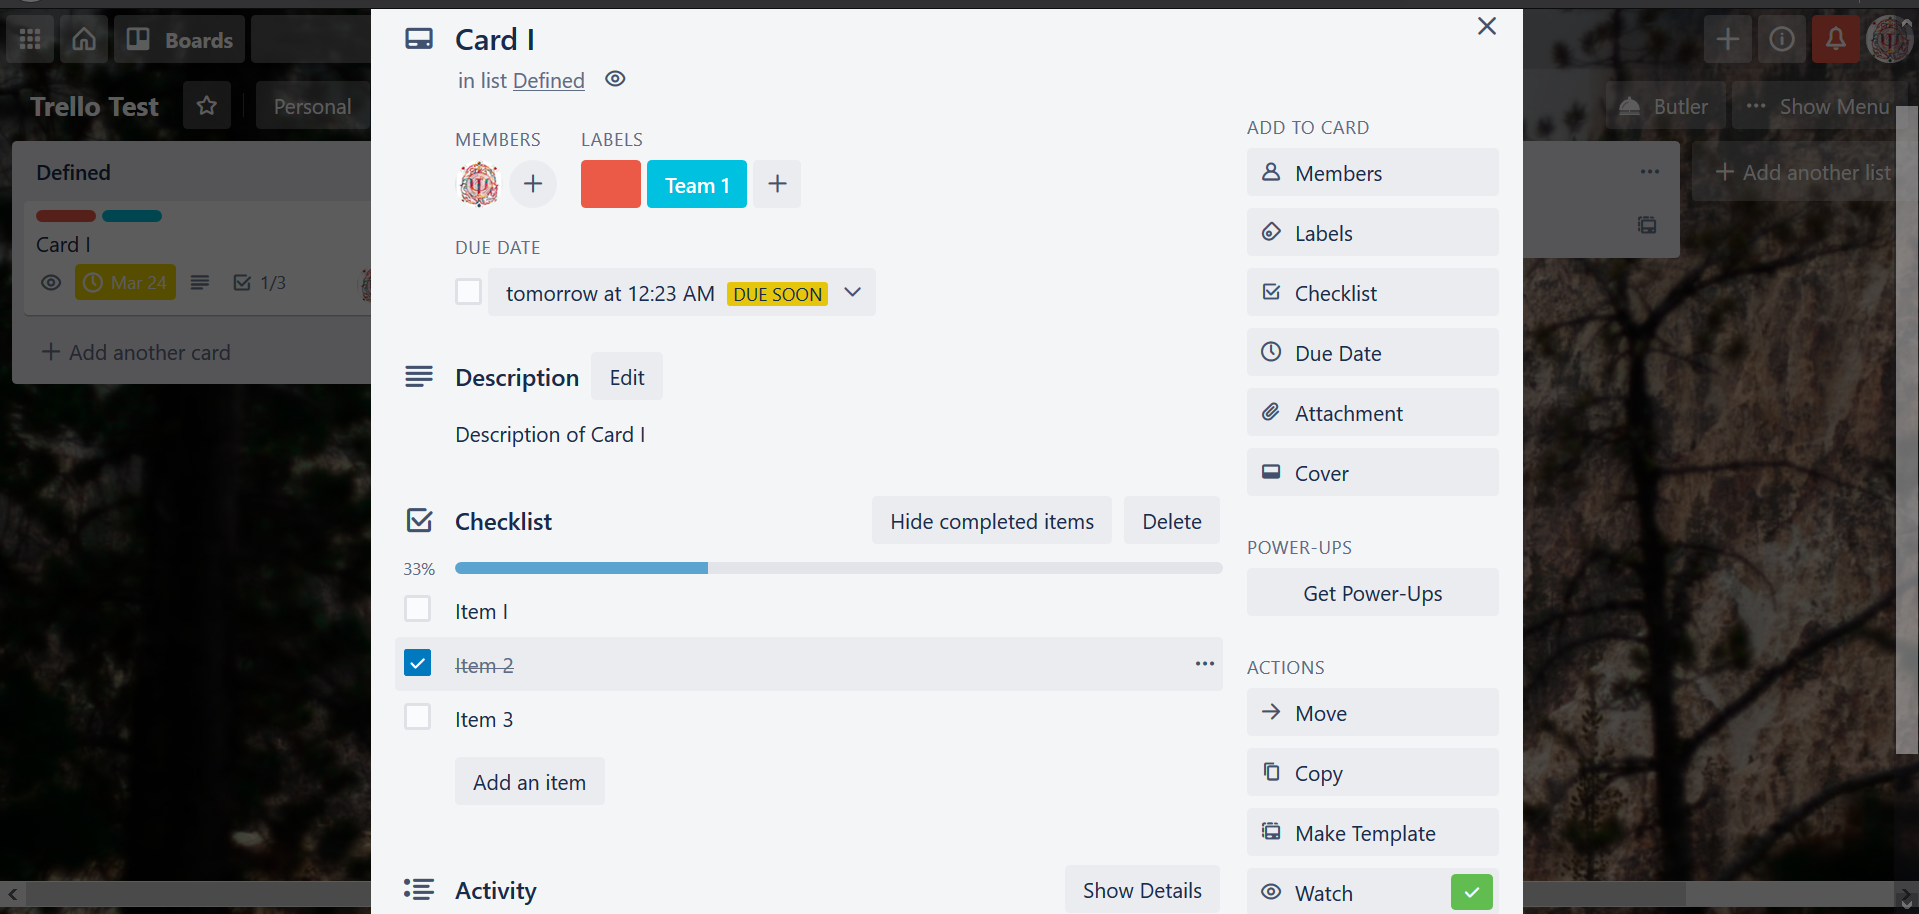
\includegraphics[width=1.0\textwidth]{images/image5.png}

\end{center}

\begin{center}


\includegraphics[width=1.0\textwidth]{images/image6.png}

\end{center}

\item
همچنین برای کارت‌ها دو طرف وجود دارد:

\begin{itemize}

\item
تحویل گیرنده (\lr{Assigner}) که عموما مسئولیت مشاهده یا \lr{watch} بر عهدهٔ وی است.

\item
تحویل دهنده (\lr{Assignee}) که در لیست اعضا نامشان آمده است.

\end{itemize}

برای هر کارت، ضرب‌الاجل یا \lr{deadline} نیز تحت عنوان \lr{due date} (زمان مقرر) مطرح می‌شود.

\begin{center}

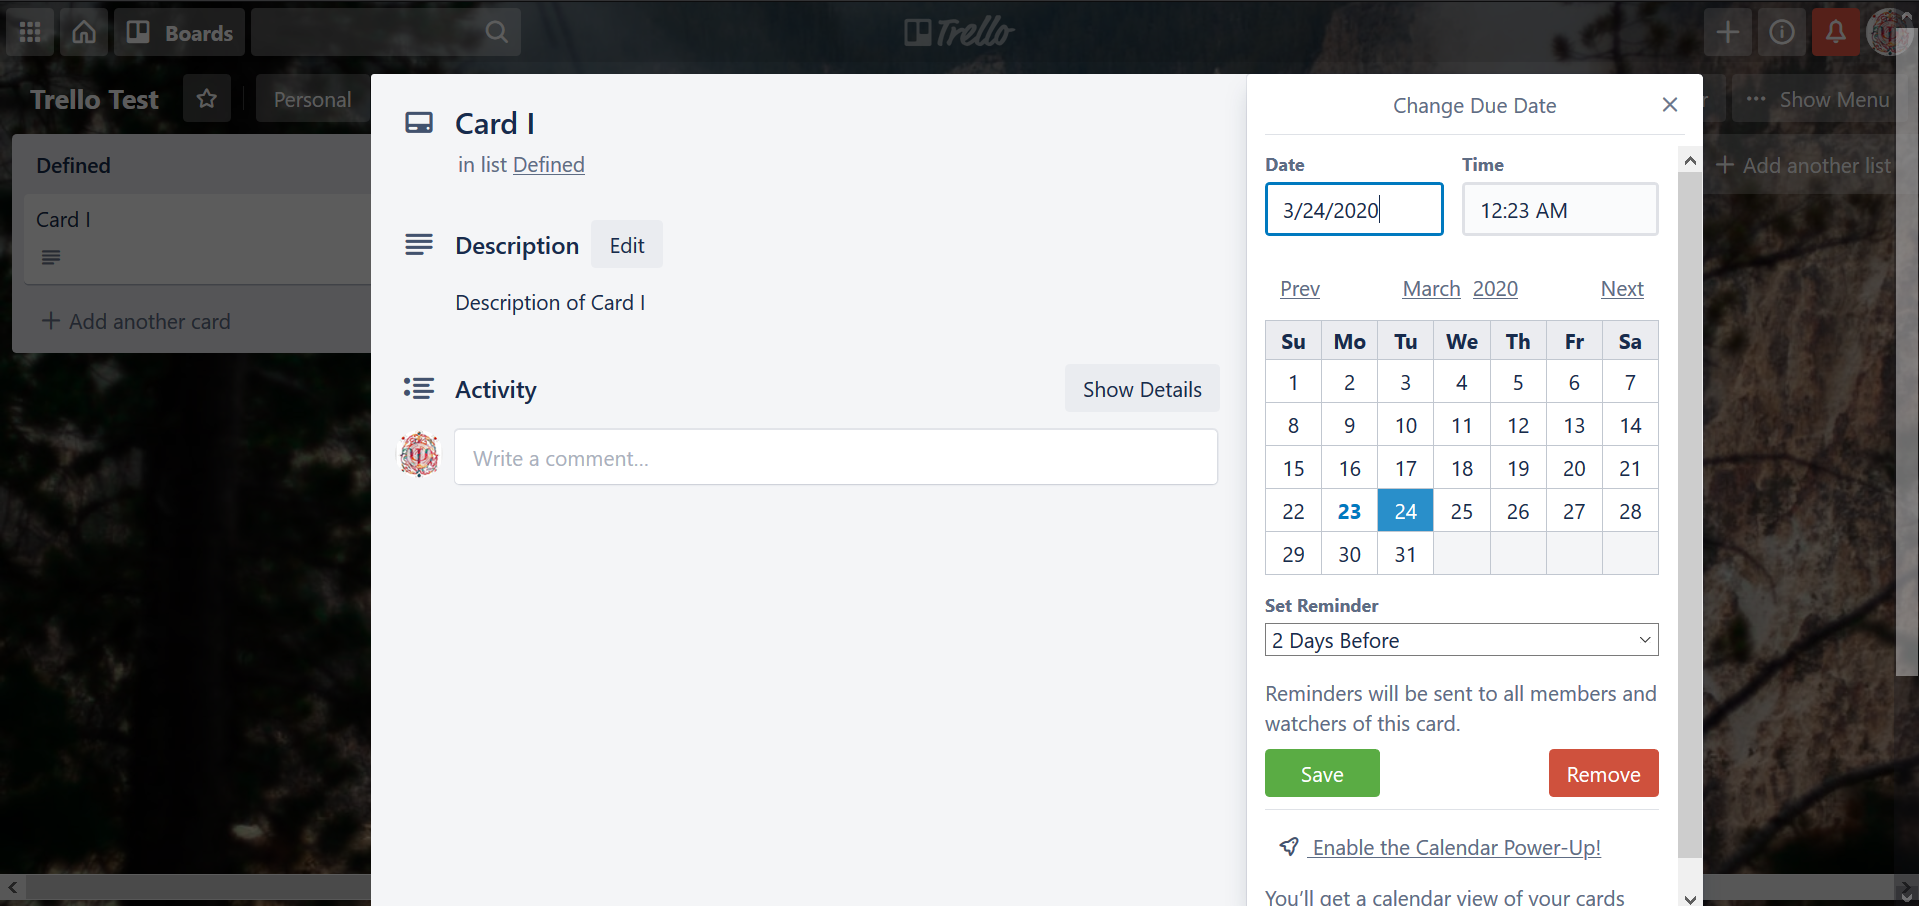
\includegraphics[width=0.8\textwidth]{images/image7.png}

\end{center}

\end{itemize}

\end{document}









